

%% AP Physics MC Questions Archive
%%----------------------------------------


%% First Law Inclines
%%----------------------------------------
\element{ap}{
\begin{question}{first-law-inclines-q01}
    Base your answer to the following question on the picture below which shows a \SI{3}{\kilo\gram} block sliding \SI{50}{\meter} down a frictionless inclined plane dropping a distance of \SI{30}{\meter}.
    \begin{center}
    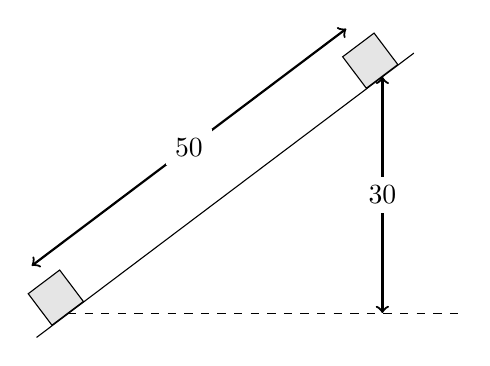
\begin{tikzpicture}
        %% Plane
        \draw (0,0) -- (37:6);
        %% Blocks
        \node[draw,rotate=37,anchor=south,minimum size=0.5cm,fill=white!90!black] (A) at (37:0.5) {};
        \node[draw,rotate=37,anchor=south,minimum size=0.5cm,fill=white!90!black] (B) at (37:5.5) {};
        %% Lables
        \draw[<->,thick] (A.north) ++(127:0.25) -- ++(37:5) node[pos=0.5,anchor=center,fill=white] {\SI{50}{\meter}};
        \draw[<->,thick] (37:5.5) --++(270:3) node[fill=white,pos=0.5,anchor=center] {\SI{30}{\meter}};
        \draw[dashed] (37:0.5) -- ++(0:5);
    \end{tikzpicture}
    \end{center}
    What is the magnitude of the normal force of the plane on the block?
    \begin{multicols}{3}
    \begin{choices}
        \wrongchoice{\SI{5}{\newton}}
        \wrongchoice{\SI{8}{\newton}}
        \wrongchoice{\SI{16}{\newton}}
      \correctchoice{\SI{24}{\newton}}
        \wrongchoice{\SI{30}{\newton}}
    \end{choices}
    \end{multicols}
\end{question}
}

\element{ap}{
\begin{question}{first-law-inclines-q02}
    A \SI{5.0}{\kilo\gram} object rests on a an inclined plane that makes an angle of \ang{30} to the horizontal.
    The net force felt by the object is most nearly:
    \begin{multicols}{3}
    \begin{choices}
        \wrongchoice{\SI{2.5}{\newton}}
        \wrongchoice{\SI{5}{\newton}}
        \wrongchoice{\SI{25}{\newton}}
      \correctchoice{\SI{50}{\newton}}
        \wrongchoice{\SI{75}{\newton}}
    \end{choices}
    \end{multicols}
\end{question}
}

\element{ap}{
\begin{question}{first-law-inclines-q03}
    The top of a \SI{50}{\meter} long inclined plane is \SI{5}{\meter} off the ground.
    If a \SI{10}{\kilo\gram} mass is at the top of this plane,
        the net force it feels is most nearly:
    \begin{multicols}{3}
    \begin{choices}
        \wrongchoice{\SI{1}{\newton}}
        \wrongchoice{\SI{5}{\newton}}
      \correctchoice{\SI{10}{\newton}}
        \wrongchoice{\SI{25}{\newton}}
        \wrongchoice{\SI{50}{\newton}}
    \end{choices}
    \end{multicols}
\end{question}
}

\newcommand{\apFirstLawInclinesQFour}{
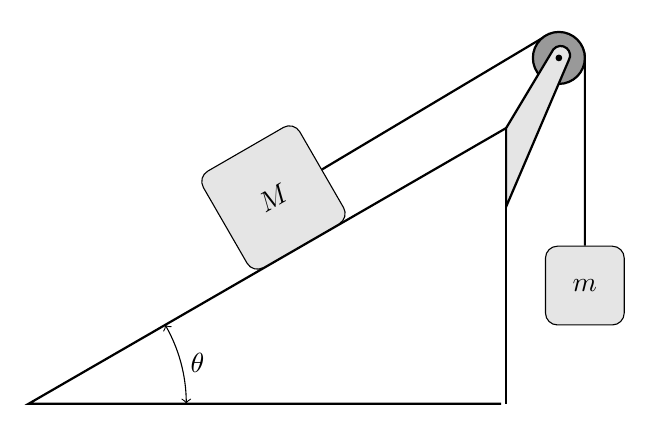
\begin{tikzpicture}
    %% Plane Floor
    \draw[thick] (0,0) -- ++(210:7) -- ++(0:6);
    \draw[<->] (210:7) ++(0:2) arc (0:30:2) node[pos=0.5,anchor=west] {$\theta$};
    \draw[thick] (0,0) -- (270:3.5);
    %% Mass
    \node[draw,fill=white!90!black,rectangle,rounded corners=1ex,minimum size=1.414cm,rotate=30,anchor=south] (A) at (210:3) {$M$};
    \node[draw,fill=white!90!black,rectangle,rounded corners=1ex,minimum size=1cm,anchor=center] (B) at (1,-2) {$m$};
    %% Rope and Pully
    \draw[thick] (A.east) -- (0.505,1.17) arc(120:0:0.33) -- (B.north);
    \draw[thick,fill=white!60!black] (0.67,0.891) circle (0.33);
    \draw[thick,fill=white!90!black] (0,0) -- (0.60,1.0) arc (140:-30:0.12) -- (0,-1) -- cycle;
    \draw[fill] (0.67,0.891) circle (1pt);
\end{tikzpicture}
}

\element{ap}{
\begin{question}{first-law-inclines-q04}
    %% Base your answers to questions 4 and 5 on the following.
    A block of mass $M$ on a frictionless ramp that makes an angle of $\theta$ to the horizontal. It is held at rest by a massless string which passes over a frictionless pulley and is attached to a block of mass $m$ as shown in the diagram below.
    \begin{center}
        \apFirstLawInclinesQFour
    \end{center}
    The normal force on the block of mass $M$ is:
    \begin{multicols}{3}
    \begin{choices}
        \wrongchoice{$\dfrac{Mg}{\cos\theta}$}
        \wrongchoice{$\dfrac{Mg}{\sin\theta}$}
        \wrongchoice{$Mg$}
      \correctchoice{$Mg\cos\theta$}
        \wrongchoice{$Mg\sin\theta$}
    \end{choices}
    \end{multicols}
\end{question}
}

\element{ap}{
\begin{question}{first-law-inclines-q05}
    %% Base your answers to questions 4 and 5 on the following.
    A block of mass $M$ on a frictionless ramp that makes an angle of $\theta$ to the horizontal. It is held at rest by a massless string which passes over a frictionless pulley and is attached to a block of mass $m$ as shown in the diagram below.
    \begin{center}
        \apFirstLawInclinesQFour
    \end{center}
    The mass $m$ is equal to:
    \begin{multicols}{3}
    \begin{choices}
        \wrongchoice{$\dfrac{M}{\cos\theta}$}
        \wrongchoice{$\dfrac{M}{\sin\theta}$}
        \wrongchoice{$M\tan\theta$}
        \wrongchoice{$M\cos\theta$}
      \correctchoice{$M\sin\theta$}
    \end{choices}
    \end{multicols}
\end{question}
}

\element{ap}{
\begin{question}{first-law-inclines-q06}
    What force is required to push a block (mass $m$) up an inclined plane that makes an angle of $\theta$ with the horizon at a constant velocity, if the coefficient of friction between the plane and the block is $\mu$?
    \begin{choices}
      \correctchoice{$mg\left(\mu\cos\theta+\sin\theta\right)$}
        \wrongchoice{$mg\mu\cos\theta$}
        \wrongchoice{$mg\left(\mu\sin\theta+\sin\theta\right)$}
        \wrongchoice{$mg\left(\mu\cos\theta+\mu\sin\theta\right)$}
        %% E is literally impossible!!
        \wrongchoice{$g\left(\mu\cos\theta+m\sin\theta\right)$}
    \end{choices}
\end{question}
}


\endinput


